\section{Zaključak}

Razvijena aplikacija omogućava jednostavno upravljanje osnovnim režimima rada
AD9850 integrisanog kola. \\
RPi se pokazao kao dobra platforma za razvoj korisničkog interfejsa generatora
funkcija i ostavlja mogućnost za lako proširenje funkcionalnosti. \\

\subsubsection{Predlozi proširenja}
U nastavku biće predloženi načini na za proširenje ovog projekta.
Implementacijom ovih predloga može se dobiti uređaj za testiranje u oblasti audio elektronike
i drugih oblasti na višim frekvencijama. \\
Većina ovih predloga zahteva projektovanje dodatnih analognih
elektronskih kola pa zbog toga njihova implementacija nije razmatrana u ovom projektu. \\

\begin{itemize}
\item \textbf{Dodavanje izlaznog pojačavača} sa mogućnosti dodavanja napona
  offset napona kako bi se obezbedili standardni naponski nivoi prisutni kod
  komercijalnih generatora funkcija (+,- 15V). \\
  Zbog relativno širokog opsega frekvencija generisanog signala (0-40MHz) ovo
  nije trivijalan zadatak i potrebno je korišćenje odgovarajućeg operacionog
  pojačavača sa dovoljno širokim frekventnim opsegom, alternativno ograničiti
  izlaznu frekvenciju na uži opseg.

\item \textbf{Softversko podešavanje ispune pravougaonog signala}. \\
  Modul korišćen u ovom projektu nema spoljni pristup ulazu internog komparatora i
  potrebno je izvršiti modifikaciju na ploči ili projektovati novu ploču.
  Potrebno je obezbediti analogni napon sa mogućnosti podešavanja softverskim
  putem, najverovatnije korišćenjem integrisanog \textbf{AD} konvertora.

\item \textbf{Proširenje projekta na Wobbler generator}. \\
  Realizovan sweep režim rada predstavlja osnovu Wobbler generatora. \\
  AD9850 je pogodan za realizaciju ovog uređaja zbog širokog opsega izlazne
  frekvencije i mogućnost brze promene frekvencije. \\
  Pored Sweep signala potrebno je obezbediti i trouglasti signal za vremensku
  bazu osciloskopa kao i potrebne pojačavače za oba signala.

\end{itemize}

\subsubsection{Slike rada}

U nastavku su okačene slike sa logičkog analizatora koje prikazuju rad uređaja.

\begin{figure}[H]
  \centering{
    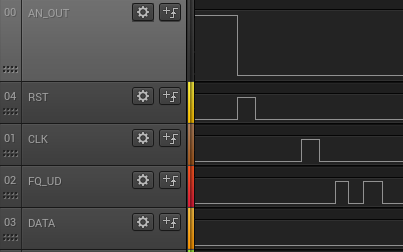
\includegraphics[width=10cm]{img/capture/rst.png}
    \caption{Reset sekvenca}
    \label{reset_seq_la}
  }
\end{figure}

\begin{figure}[H]
  \centering{
    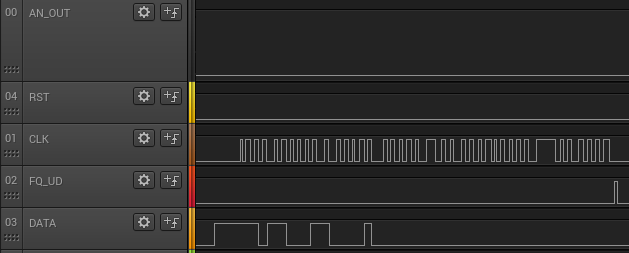
\includegraphics[width=12cm]{img/capture/data_write.png}
    \caption{Serijski upis}
    \label{serial_write_la}
  }
\end{figure}

\begin{figure}[H]
  \centering{
    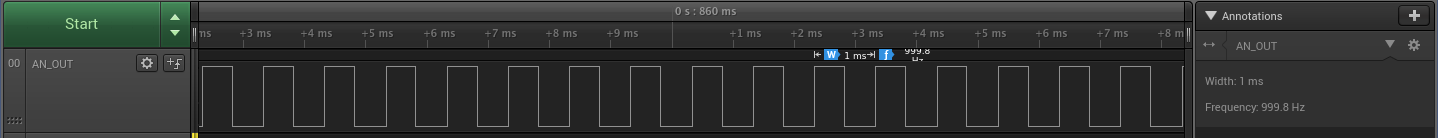
\includegraphics[width=18cm]{img/capture/an_out1khz.png}
    \caption{Run režim, frekvencija 1kHz}
    \label{run_1khz_la}
  }
\end{figure}

\begin{figure}[H]
  \centering{
    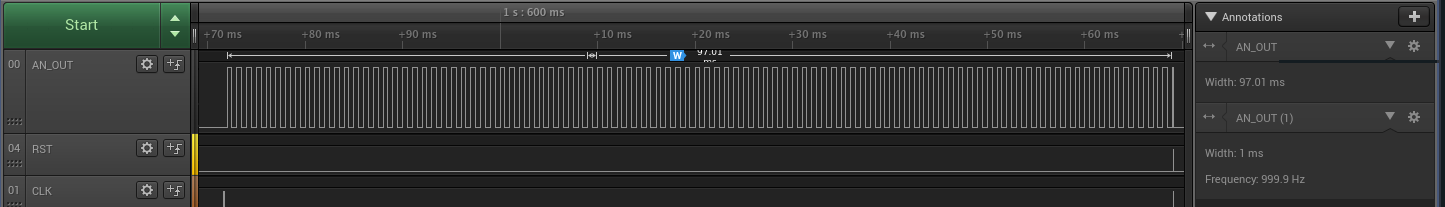
\includegraphics[width=18cm]{img/capture/run_for_100ms_1khz.png}
    \caption{Run for režim, 1kHz 100ms}
    \label{run_for_la}
  }
\end{figure}

\begin{figure}[H]
  \centering{
    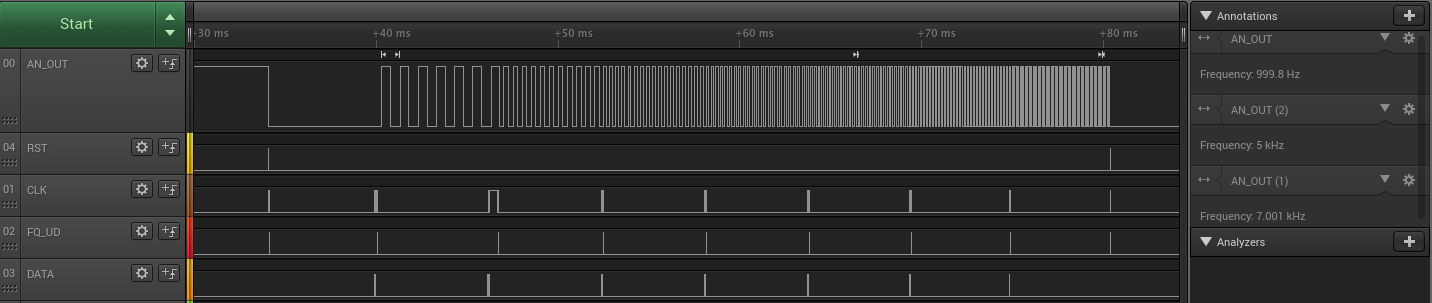
\includegraphics[width=18cm]{img/capture/sweep_1000_8000_1000_5.png}
    \caption{Sweep režim, 1kHz do 7kHz, korak od 1kHz i vreme koraka 50ms}
    \label{sweep_la}
  }
\end{figure}